 \label{chap:Conceptions}
This chapter contains 5 sections. Each section is dedicated to present a concept or tool that is strongly related to the proposals of our project. These concepts or tools include AST (abstract syntax tree), shared library and static library, ABI (application binary interface), FFI (forgien function interface) and SWIG (Simplified Wrapper and Interface Generator).

\section{Abstract Syntax Tree}

\paragraph{Why do we need AST?}

Imagine that you need to implement a new language name T (target language), and there exist already another language name S (source language), which has some functionalists that you need in language T. What will you do? Yes, translate language S into T so that you don't need to reinvent the wheels. And shall we build a source-to-source translator directly? The answer is, it's possible for you to do so, but we can do better. Consider the situation that you need to implement more than one new language namely T1, T2... from more than one source language namely S1, S2... It would be painful if you build a translator to do the source-to-source translation according to different concrete syntax of each language. What we can do is to use the language independent abstract syntax tree to represent the essential logic of different program. According to Joel Jones\cite{Joel-Jones-03}, there are systems automatically generate AST implementations, such as Zephyr ASDL\cite{Daniel-97} and Eli\cite{Robert-92}. 


\paragraph{What is AST?}

As the name implicated, AST is a tree representation of source code syntax in an abstract level. We say this representaion is "abstract" because the tree does not show all details, such as semi-colons to terminate statements or commas to separate function argument in the real syntax, but the essential characteristics of the structure.\cite {Joel-Jones-03}. Plus, ASTs omit tree nodes representing unary productions in the grammar, because information like that 
"directly represented in ASTs by the structure of the tree"
\cite {Joel-Jones-03}.

Figure \ref{fig:AST-example} is an example of AST generated from Euclidean algorithm from Wikipedia \footnote{https://en.wikipedia.org/wiki/Abstract\_syntax\_tree}. It's clear that only abstract logic of the algorithm is shown in an AST and there isn't any hint of a specific programming language.       

\begin{figure}[h!]
  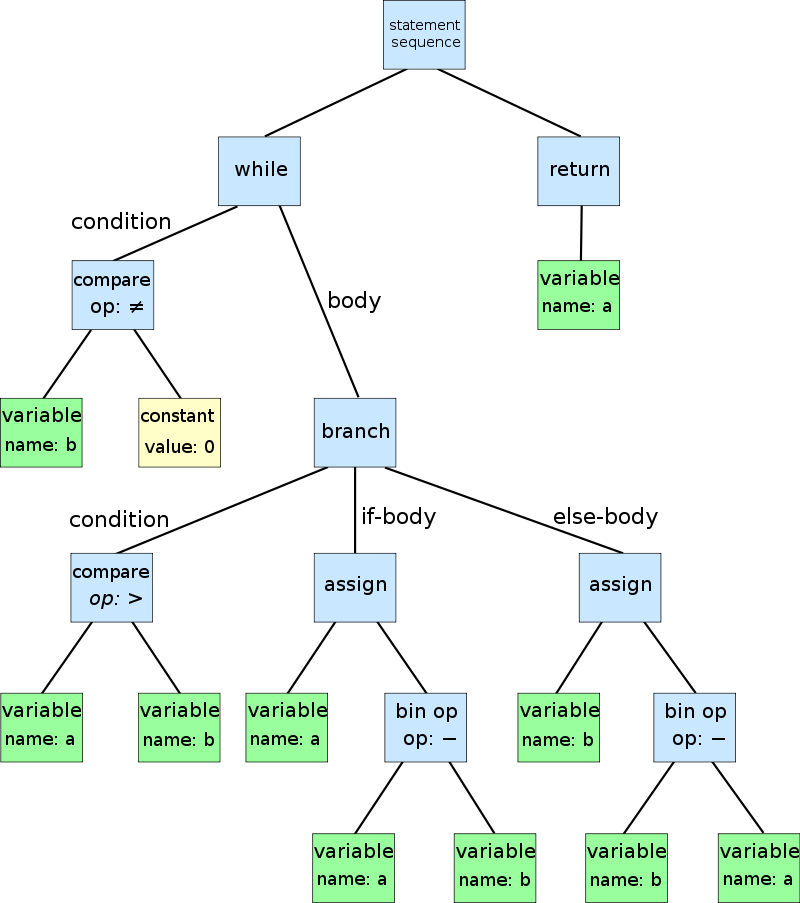
\includegraphics[scale=0.25]{Images/AST.png}
  \caption[An abstract syntax tree for the following code for the Euclidean algorithm:]%
    {An abstract syntax tree for the following code for the Euclidean algorithm}
 
  \begin{minted}{python}
while b Not Equal to 0
    if a > b
    a := a - b
    else
    b := b - a
return a
\end{minted}
  \label{fig:AST-example}
\end{figure}


\section{Library}
\paragraph{Why library?}
Firstly, let's just pick a routine that's really simple with piece of code that's highly used and one good example is printing something on standard out or printing something to the terminal. If
almost every program needs that utilize printing something to the screen, do you think every single developer writes their own version of the print function? Actually every developer could write their own version of print screen but it wouldn't really be a good use of their time. No one is here to reinvent the wheel when a lot of applications use common functionality like, in this example, common functionality is just printing something to the screen. Well, when this happens, a lot of common functionality and common code should be packaged up into what we call the library.

\paragraph{What exactly is a library?}
First thing is that a library itself is just file. Nothing more nothing less. It's just a file persisted on your computer and consists of ones and zeros like every other file\cite{Wexelblat-81}. The major separating factor that we have to understand between the library and every other application is that you cannot execute a library. Libraries don't actually execute. Applications execute but they utilize libraries\cite{Wexelblat-81}. 


There are two basic ways of how libraries work. One is called shared library and the other called static library.
	
	\subsection{Shared Library}
	If you use linux these are the ".so" files. If you use windows these are ".dll" files and if you use mac these are ".dylib" files. Different extensions across different platforms. 
	
	If our application utilizes a shared library, it means the application is going to reference that library exactly when it needs the reference\cite{Hart-05}\cite{Rector-05}. It happens in its running time. So let's just take an example of this. When your application needs to print something to the screen. It is going to reference a shared library on the computer that knows how to print something to the screen and let that shared library handle it. None of that printing code lives in our application. They actually lives in that shared library. So what's the one major contingency for using the shared library is they have to be available during the running time of our application. Applications actually just gonna straight-up crash if the shared library isn't available. So this is creating a really tight dependency between the two\cite{Hart-05}\cite{Rector-05}. 
	
	\subsection{Static Library}
	Static libraries on Linux have the .a file extension and on Windows have the .lib file extension\footnote{http://stackoverflow.com/questions/6422478/linking-a-lib-and-def-files}.
	
	Static library is the complete opposite of a shared library. Our program is going to utilize a static library at compile time, which is before running time\footnote{http://tldp.org/HOWTO/Program-Library-HOWTO/static-libraries.html}. Something has to be compiled before you can even run it. Utilizing a static library, we take exactly what we need from the static library and we literally copy all the code we need and move it into our application so our application has it. It's just like a copy and paste.
	
	\subsection{Pops and Cons}
    The major pro with the shared library is that since you don't do this copy and pasting, all you do is reference the library's when you need it. That keeps your application really really small. While it would be very inconvenient to manage libraries dependency if your application relays on hundreds or thousands of shared libraries.    
    
    The major pro with the static shared library is that dependencies are already compiled into your program at compile-time. So when you you just say here you go here's the application and that's all you need to run it. While the cost is your application size could be very large.




\section{Application Binary Interface}

    \paragraph{What's an ABI?}
    An application binary interface (ABI) describes the interface between two program modules, one of which is often a library or operating system  and the other is an application, at the binary code level. \footnote{https://en.wikipedia.org/wiki/Application\_binary\_interface}
    Thus, it is ABI that actually determines the binary compatibilite between an application and a system.\footnote{http://abicheck.sourceforge.net/}\newline    
   Accroding to \cite{ALTERA-14}, ABI describes:   \begin{itemize}
      \item  How data is arranged in memory
      \item  Behavior and structure of the stack
      \item Function calling conventions
    \end{itemize}
    
    \paragraph{Why do we need ABI?}
    Do you still remember that we have talked about library before? For our project, in order to use the library generated from C++ by JavaScript, we need a mechanism or a standard telling JavaScript how to use those binary code in that C++ library. That's when we need the ABI! Since ABI determinates something like how functions arguments are passed and return values retrieved; the sizes, layout, and alignment of data types; how to manager registers and stacks ect \cite{ALTERA-14}, if our C++ library and JavaScript file as well as our operate system follow the same ABI standard, they can perfectly cooperate in machine code level.
    
  
\section{Foreign Function Interface}

    Till now, we have talked about library, the structure mechanism of using a library (ABI). It's time to use that library from within JavaScript. One possible way to do that is using the FFI model of Node. Firstly, let's see what's FFI.
    
    \paragraph{What is FFI?} FFI refers to the ability for code written in one language, namely "host language," such as JavaScript, to access and invoke functions written in another language, namely the "guest language," such as C++\cite{Sigbjorn-99}.The reason why we call those functions "foreign" is because they come from another language and environment.\cite{Matthias-Grimmer-14}
    
    FFI access directly a library's binary code, which means it uses standard ABI to invoke functions in the library.
    
    \paragraph{Why FFI is good?} John Croisant, an experienced Ruby programmer, has shared 3 ideas of how to library written in lower-level languages, like C, within high-level languages, like Ruby.\footnote{\label{note1}https://spin.atomicobject.com/2013/02/15/ffi-foreign-function-interfaces/} They are:\newline
   
        \begin{itemize}
            
            \item \textit{1 Port all or part of the library to your language of choice.}
            \item \textit{2 Write an extension in C code to bridge the gap between the library and your language.}
            \item \textit{3 Wrap the library using your language's foreign function interface (FFI) support. }
           \textsuperscript{\ref{note1}}\newline
        \end{itemize}
    
    So why FFI is the good? According to John, the major pops of FFI is its convenience to write and maintain compared with a C extension, its portability across platforms and language implementations, and it is easier for users to install. \textsuperscript{\ref{note1}}
    
    
    \paragraph{Node FFI}
    As you already know what FFI is, you can surely guess what Node FFI can do. I mention it here because on of the possible solution of our project is highly depending on this tool. Below is the definition given by the official documentation of Node FFI \textit{"node-ffi is a Node.js addon for loading and calling dynamic libraries using pure JavaScript. It can be used to create bindings to native libraries without writing any C++ code."} \footnote{https://github.com/node-ffi/node-ffi}


\section{SWIG}
    Finally, we come to the last conception of this chapter! Let's go.
    \paragraph{What is SWIG?} The full name of SWIG is simplified wrapper and interface generator. It's a software that used to translate c and c++ files into scripting language or other languages. In the other word, it gives us the ability to call c and c++ files or programs or libraries from within other languages\footnote{http://www.swig.org/}.
    In fact, part of the job that SWIG does is quiet similar to Node FFI. They all wrap functions written in low-level languages in order to invoke them in high-level languages. Plus, SWIG goes further. It can automatically generate shared libraries from source code and solves the problem of name mangling. Maybe there are something more. We will see. 
    
    \paragraph{Version 3.0 of SWIG}
    It's worth noting that from Version 3.0 of SWIG\footnote{http://waywardmonkeys.org/2014/10/01/swig-and-javascript-part-one/}, it began to support JavaScript. And that's how comes our second proposal. 


\begin{comment}
  A clear view of the advantages and disadvantages of the partial solutions found in the literature can be summarised by one or several tables (cf.\ table~\ref{tab:ProposalsComparison}) where a number of important criteria have been introduced and described.

Note that all figures, tables, and algorithms must be put into their corresponding floating environments, captioned, referenced from the main text, and sourced if they have been copied from previous work.
\end{comment}
  



\section{Conclusion}
In this chapter, we have gone through 4 basic conceptions in computer science. They are respectively AST, Library, ABI and FFI. Moreover, we have introduced two tools, on which our proposal of this project will largely depend. One is Node FFI and the other is SWIG. In next chapter, general ideas of two proposals, namely possible solutions, of our project will be given.  
  
%--------------------------------------------------------------------------------

% \part{Proposals} % Commet it out if this has been done for the state-of-the-art
% \label{part:Proposal